\documentclass[12pt]{article}
\usepackage{a4wide}
\usepackage{amsmath,amssymb}
\usepackage{bm}
\usepackage[colorlinks]{hyperref}
\usepackage{listings}
\usepackage{graphicx}
\usepackage{pgfgantt}
\usepackage{url}
\UseRawInputEncoding
\usepackage{cite}
\usepackage{mathptmx}
\usepackage{times}
\usepackage{fancyhdr}
\usepackage{amsmath}
\usepackage[toc,page]{appendix}
\usepackage{color}
\usepackage{captcont}
\usepackage{hvfloat}
\usepackage{subcaption}
\usepackage{caption}
\usepackage[section]{placeins}
\usepackage{rotating}
\usepackage{tcolorbox}
\usepackage{adjustbox}
\usepackage{blindtext}
\usepackage{booktabs}
\usepackage{float}
\usepackage{lscape}
\usepackage{gensymb}
\usepackage{ragged2e}
\usepackage[center]{titlesec}
\usepackage{sectsty}
\usepackage{lipsum}
\usepackage{afterpage}
\usepackage{parskip}
\usepackage{nomencl}
\makenomenclature
\usepackage{siunitx}
\usepackage{forest}
\renewcommand{\figurename}{Fig.}
\usepackage{indentfirst}
\setlength{\parindent}{1cm}
\usepackage [english]{babel}
\addto\captionsenglish{\renewcommand{\figurename}{Fig. }}
\usepackage [autostyle, english = american]{csquotes}
\usepackage{nameref}
\MakeOuterQuote{"}
\oddsidemargin0cm
\topmargin-2cm     %I recommend adding these three lines to increase the 
\textwidth16.5cm   %amount of usable space on the page (and save trees)
\textheight23.5cm 
\usepackage[english]{babel}
\usepackage{setspace}
\usepackage[margin=20mm,labelfont=bf]{caption}
\usepackage[left=20mm, right=20mm, top=20mm, bottom=20mm]{geometry}
\usepackage{amssymb}
\usepackage[section] {placeins}
\usepackage{verbatim}
\usepackage{wrapfig}
\usepackage{mwe,tikz,pgfplots}
\tikzset{boximg/.style={remember picture,red,thick,draw,inner sep=0pt,outer sep=0pt}}
\usetikzlibrary{shapes}
\usetikzlibrary{spy}
\usetikzlibrary{automata,positioning}
\usetikzlibrary{arrows,calc,shapes.geometric}


\newcommand{\vect}[1]{\hat{\boldsymbol{#1}}}
\title{Report V1}
\usepackage{minted}
\begin{document}
    \maketitle

\tableofcontents

\section{Introduction}
La pratique régulière d’activités physiques comporte de nombreux bénéfices tel 
qu' une amélioration de la santé mentale ,la prévention des maladies cardiovasculaire , limiter la prise  de poids et bien d'autres . 

Cependant, on observe un déclin de la pratique d’activités physiques.
il apparaît primordia d’encourager les jeunes à maintenir une activité physique ou devenir plus actif , c'est dans cette optique que s'inscrit ce projet . 



\subsection{Sport et sciences sociales}

Créée en 1979 par Bernard Michon à Strasbourg ,l’unité de recherche Sport et sciences sociales
demeure la seule unité de recherche STAPS du Grand Est et est reconnue comme une structure de recherche incontournable  en sciences sociales du sport dans le paysage français et européen.
Regroupant plus de 20 chercheurs (titulaires et associés) et 17 doctorants, elle réalise  des	ouvrages	et	des	articles de	référence (plus	de	174	publications).



\subsection{Main Objectives}

The objective of this work is to identify profiles of practitioners based on positive or negative qualifiers, i.e., to assign a profile to each cluster of the data and to estimate the strength of these profiles, i.e., the number of clusters or profiles that are most representative of the data.


\subsection{Specific Objectives}
Nous allons d'abord effectuer un prétraitement des données par la renormalisation des données , la suppression des valeurs aberrantes,  compléter ou  supprimer les valeurs manquantes, puis pour analyser les données nous utiliserons différents algorithmes tels que : K-means, analyse en composantes principales, arbres de décision. Enfin, nous testerons la solidité de notre cluster en utilisant des algorithmes de classification tels que : la régression logistique, la régression linéaire,...


We will first perform a preprocessing of the data by renormalizing the data, removing outliers, completing or removing missing values, then to analyze the data we will use different algorithms such as: K-means, principal component analysis, decision trees. Finally, we will test the robustness of our cluster by using classification algorithms such as: logistic regression, linear regression,...



Le diagramme de Gantt ci-dessous nous donne un aperçu rapide de l'organisation du travail dans le temps .

\begin{ganttchart}[
  hgrid,x unit=1.5mm,
  hgrid style/.style={draw=black!5, line width=.75pt},
  vgrid={*{6}{draw=none},dotted},
  time slot format=little-endian,
]{1-04-2022}{27-05-2022}
  \gantttitlecalendar{ month=shortname,week=4} \\
  \ganttgroup{Report V0}{1-04-2022}{5-04-2022}\\
  \ganttbar{data pre-processing}{5-04-2022}{30-04-2022}\\
  \ganttbar{clustering methods}{5-04-2022}{10-05-2022}\\
  \ganttbar{Validation}{5-04-2022}{22-05-2022}\\
  \ganttgroup{Report V1}{5-04-2022}{22-05-2022}\\
  \ganttbar{data pre-processing}{5-04-2022}{30-04-2022}\\
  \ganttbar{clustering methods}{5-04-2022}{10-05-2022}\\
  \ganttbar{Validation}{5-04-2022}{22-05-2022}\\
  \ganttgroup{Report Vfinale}{22-05-2022}{27-05-2022}\\
\end{ganttchart}



\section{Description of raw data}

Le dataset contient des informations personnels sur les lycéens qui sont au total 1070 tel  que leur initial, le Lycée, le sexe , le choix d'étude ,le travail des parents et le support des parents ainsi que la date de naissance , la  morphologie de la personne ( la taille et le poids ) . Une vingtaine des  variables mesurent la nature de la motivation par exemple la jouissance , l'affiliation , la condition physique  et  le dégré de motivation tel que SIMS intrinsic et SIMS external regulation . 

Enfin le reste des  variables (71)  sont obtenu de la manière suivante :
on pose une question : "En EPS, quel est le sport que vous avez le plus apprécié ?".

Puis on lui indique :
"Nous allons maintenant te présenter des mots qui vont te permettre de décrire ton ressenti par rapport à ce sport. Votre travail consiste à indiquer, le plus rapidement possible, si vous êtes d'accord ou non avec ces propositions en cliquant sur oui ou non.
Le temps de réponse a été pris en compte dans chaque réponse. Si ce temps est court, cela signifie que le terme semble évident.
Par exemple, si le sport est "le football", l'élève pourra répondre "oui" rapidement au qualificatif "plaisir", "non" rapidement au qualificatif "beauté".

Les réponses possibles à chaque question sont "oui", "non", "je ne sais pas". Lorsque la réponse à une question est "oui", la valeur du temps est positive, négative dans le cas de "non" et zéro dans le cas de "je ne sais pas".



The dataset contains personal information about the students such as their initial, high school, gender, choice of study, parents' work and parents' support as well as date of birth, body shape (height and weight). Twenty variables measure the nature of motivation such as enjoyment, affiliation, physical condition and the degree of motivation such as SIMS intrinsic and SIMS external regulation. 

Finally the rest of the variables (71) are obtained in the following way:
we ask a question: "In PE, what is the sport that you enjoyed the most?

Then one indicates to him:
"We are now going to present you with words that will allow you to describe your feelings about this sport. Your job is to indicate, as quickly as possible, whether you agree or disagree with these propositions by clicking on yes or no.
The response time has been taken into account in each answer. If this time is short, it means that the term seems obvious.
For example, if the sport is "soccer", the student could answer "yes" quickly to the qualifier "fun", "no" quickly to the qualifier "beauty".

The possible answers to each question are "yes", "no", "I don't know". When the answer to a question is "yes", the time value is positive, negative in the case of "no" and zero in the case of "I don't know".






\begin{figure}[h]
\begin{center}
\includegraphics[scale=0.5]{donnée_brute.png} 
\caption[]{ Raw \ data}
\end{center}
\end{figure}


\section{Preprocessing}

\subsection{Preprocessing Method}

Dans ce projet , Les valeurs manquantes ont été mise à zéros en supposant que le qualificatif n'intéresse pas les étudiants concernés et qu'ils auraient pu  répondre : "je ne sais pas".
Pour la gestion des valeurs aberrantes , celles qui sont  supérieur à 5*écart-type ont été mise à zéros en fin de ne pas impacter le poids donnée à chaque  mot. L'écart-type a été calculé en utilisant les données non signées dans le but de réduire les valeurs extrême et éviter la possible compensation des valeurs.
Les étudiants ayant répondu "je ne sais pas" à toutes ces questions n'ont pas été considéré dans la suite du projet .  
La normalisation a été faite par ligne dans le but de conserver ce qui est "important" pour chaque personne. 



In this project, the missing values have been set to zero assuming that the qualifier does not interest the students concerned and that they could have answered: "I don't know".
For the management of the outliers, those which are higher than 5*standard deviation have been set to zero in order not to impact the weight given to each word. The standard deviation was calculated using the unsigned data in order to reduce the extreme values and avoid the possible compensation of the values.
The students who answered "I don't know" to all these questions were not considered in the rest of the project.  
The normalization was done by line in order to keep what is "important" for each person. 


\subsection{Results of processed data}

\begin{figure}[h]
\begin{center}
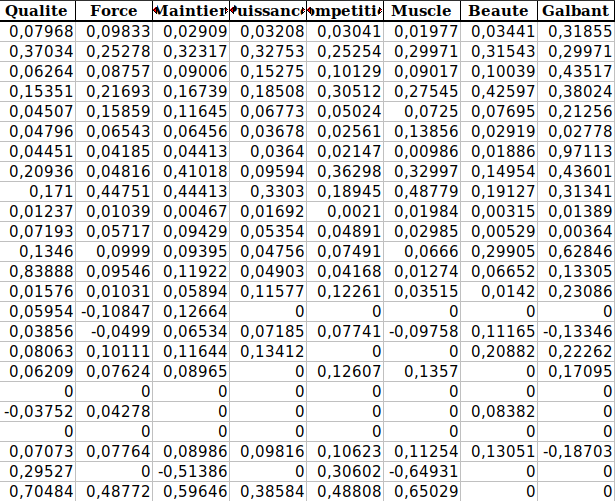
\includegraphics[scale=0.7]{donnée_nettoyé.png} 
\caption[]{Data \ processed }
\end{center}
\end{figure}



Les mots les plus "importants"  et les moins "importants" pour chaque personne sont respectivement proche de soit 1 ou de -1 . Ceux qui  sont  moins "importants" sont proches de zero.

Le jeu de données nettoie contient 1050
lycéens et 71 caractéristiques.

The most "important" and least "important" words for each person are respectively close to either 1 or -1 . Those which are less "important" are close to zero.

The cleaned dataset contains 1050
students and 71 features.


\section{Clustering} 


\subsection{Principal component analysis}

L'analyse en composantes principales est une méthode de la famille de l'analyse des données et plus généralement de la
statistique multivariée, qui consiste à transformer des variables liées entre elles (dites « corrélées » en statistique) en nouvelles variables decorrélées les unes des autres. Ces nouvelles variables sont nommées « composantes principales » ou axes principaux. Elle permet au statisticien de résumer l'information en réduisant le nombre de variables.

Dans notre projet, nous allons utiliser ACP pour réduire la dimension des données en quelques variables et garder les données les plus importants. 

Pour déterminer le nombre de composante optimale , nous avons utiliser la fonction suivante dans Rstudio.


Principal component analysis is a method of the data analysis family and more generally of multivariate statistics, which consists in transforming
multivariate statistics, which consists in transforming variables that are linked to each other (called "correlated" in statistics) into new variables that are decorrelated from each other. These new variables are called "principal components" or principal axes. It allows the statistician to summarize information by reducing the number of variables.

In our project, we will use PCA to reduce the size of the data to a few variables and keep the most important data. 

To determine the number of optimal components, we use the following function in Rstudio:

\begin{lstlisting}
fviz_eig(res.pca, addlabels = TRUE, ylim = c(0, 50))
\end{lstlisting} 

Cette fonction permet d'avoir le graphique des valeurs propres.Les valeurs propres mesurent la quantité de variance expliquée par chaque axe principal.Les valeurs propres sont grandes pour les premiers axes et petits pour les axes suivants.

The eigenvalues measure the amount of variance explained by each principal axis. The eigenvalues are large for the first axes and small for the following axes.


\newpage



\begin{figure}[H]
\begin{center}
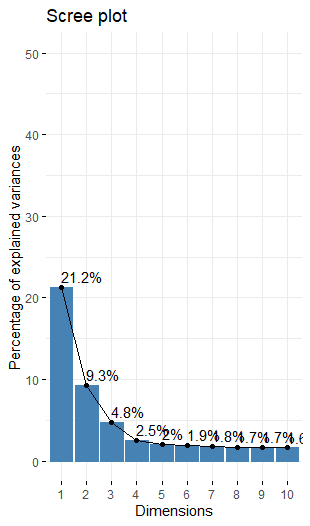
\includegraphics[scale=1.4]{ACP_1.png} 
\caption[]{\ }
\end{center}
\end{figure}

D'après le graphique ci-dessus, nous pourrions vouloir nous 
arrêter à la cinquième composante principale  car la variation est moindre après la cinquième.

Cependant 39.79760 \% des informations (variances) contenues
dans les données sont retenues par les 5  premières composantes principales.


According to the graph above, we might want to stop at the fifth principal component 
stop at the fifth principal component because the variation is less after the fifth.

However 39.79760 \% of the information (variances) contained in the data is retained by the
in the data is retained by the first 5 principal components.


Les graphique ci-dessous montre le top 30 des variables contribuant le plus aux 5 composantes principales. 
Les lignes en pointillé rouge, sur les graphiques, indique  la valeur  contribution moyenne.
 
 The graphs below show the top 30 variables contributing the most to the principal components. 
The red dotted lines on the graphs indicate the average contribution value.

\begin{figure}[H]
\begin{center}
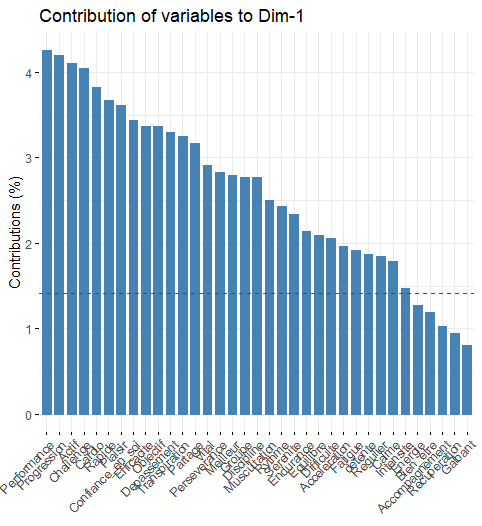
\includegraphics[scale=1.3]{ACP_2.png} 
\caption[]{\ }
\end{center}
\end{figure}


\begin{figure}[H]
\begin{center}
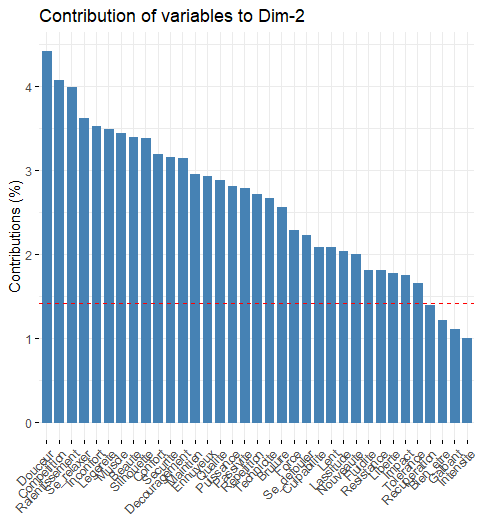
\includegraphics[scale=1.3]{ACP_3.png} 
\caption[]{\ }
\end{center}
\end{figure}


\begin{figure}[H]
\begin{center}
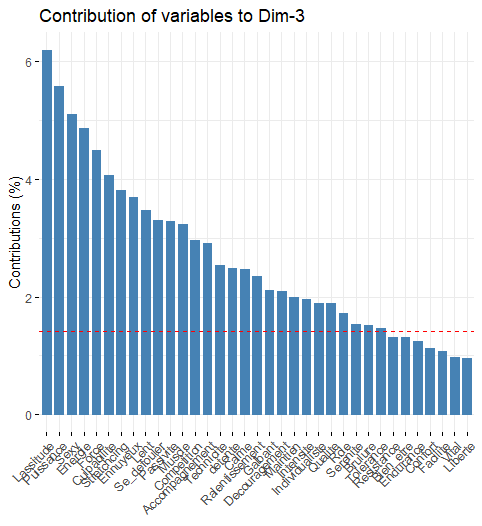
\includegraphics[scale=1.3]{ACP_4.png} 
\caption[]{\ }
\end{center}
\end{figure}


\begin{figure}[H]
\begin{center}
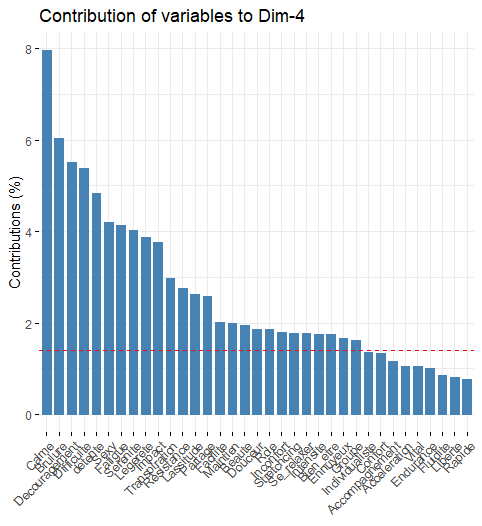
\includegraphics[scale=1.3]{ACP_5.png} 
\caption[]{\ }
\end{center}
\end{figure}


\begin{figure}[H]
\begin{center}
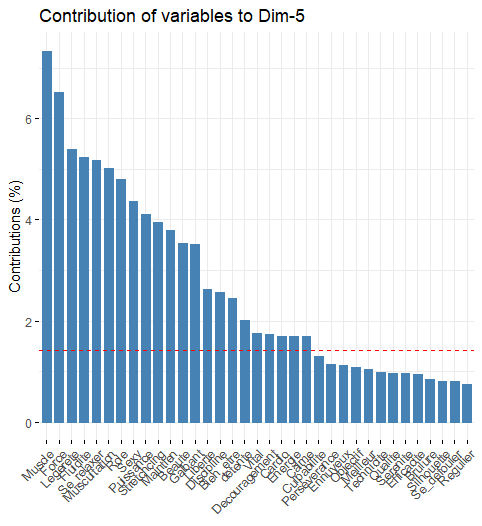
\includegraphics[scale=1.3]{ACP_6.png} 
\caption[]{\ }
\end{center}
\end{figure}


Les variables les moins importants  sont les suivantes : "Recuperation" et  "Facilité".

The least important variables are :
"Recuperation" et  "Facilité".

\newpage   


\subsection{Hierarchical Clustering on Principal Components} 


Pour réaliser le clustering, nous allons utilisé  Hierarchical Clustering on Principal Components( HCPC) .
Cette méthode permet de combiner les trois méthodes standards utilisées dans les analyses de données multivariées :

Méthodes en composantes principales (PCA, CA, MCA, FAMD, MFA),
Regroupement hiérarchique et
Clustering de partitionnement, en particulier la méthode des k-moyennes.



L'algorithme de la méthode HCPC a 4 principales étapes :

1) Effectue une ACP. Choisisse le nombre de dimensions à retenir en spécifiant l’argument ncp. Dans notre cas ,la  valeur est 5.

2) Applique la classification hiérarchique sur le résultat de l’étape 1.

3) Choisisse le nombre de groupes en fonction du dendrogramme obtenu à l’étape 2. Un partitionnement initial est effectué.Dans notre cas ,la  le nombre de groupes est 3.

4) Effectue le k-means pour améliorer le partitionnement initiale obtenu à l’étape 3.


Voici les lignes de codes principales pour :



To make the clustering, we will use Hierarchical Clustering on Principal Components (HCPC).
This method combines the three standard methods used in multivariate data analysis:

Principal Component Methods (PCA, CA, MCA, FAMD, MFA),
Hierarchical clustering and
Partitioning clustering, in particular the k-means method.


The HCPC method algorithm has 4 main steps:

1) Performs a PCA. Selects the number of dimensions to retain by specifying the argument ncp. In our case, the value is 5.

2) Apply the hierarchical clustering on the result of step 1.

3) Choose the number of groups according to the dendrogram obtained in step 2. In our case, the number of groups is 3.

4) Performs the k-means to improve the initial partitioning obtained in step 3.

Here are the main lines of code for :

\begin{lstlisting}

res.pca <- PCA(data_base , ncp = 5 ,graph = TRUE)
res.hcpc <- HCPC(res.pca,nb.clust=3,consol=FALSE,graph=TRUE)

plot(res.hcpc,choice = "tree")
plot(res.hcpc,choice = "map", draw.tree = FALSE)
plot(res.hcpc,choice = "3D.map")
catdes(res.hcpc$data.clust,ncol(res.hcpc$data.clust))

\end{lstlisting}

\begin{figure}[H]
\begin{center}
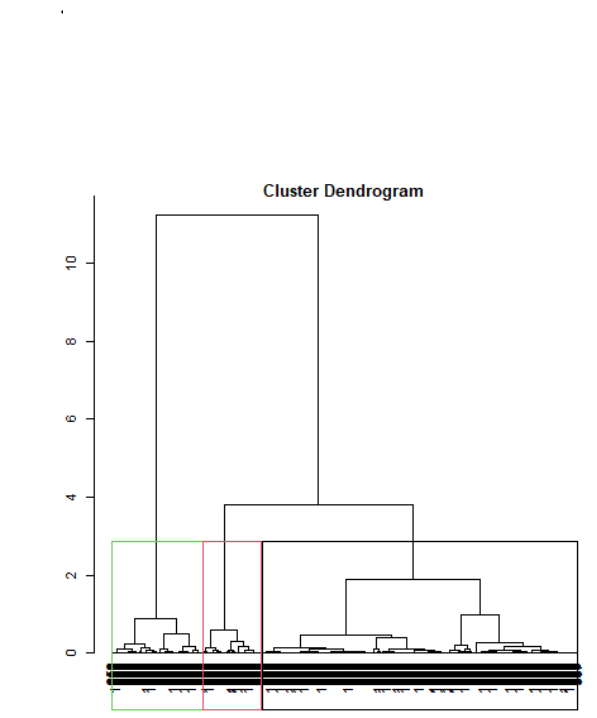
\includegraphics[scale=0.65]{classification_1.png} 
\caption[]{Hierarchical \ tree}
\end{center}
\end{figure}


\begin{figure}[H]
\begin{center}
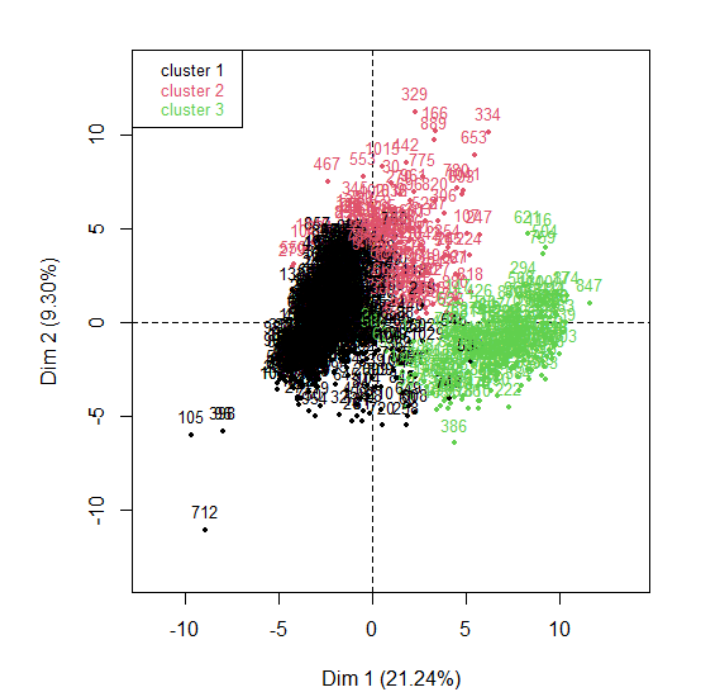
\includegraphics[scale=0.7]{classification_2.png} 
\caption[]{Ascending \ Hierarchical \ Classification \ of \ the \ individuals }
\end{center}
\end{figure}

\begin{figure}[H]
\begin{center}
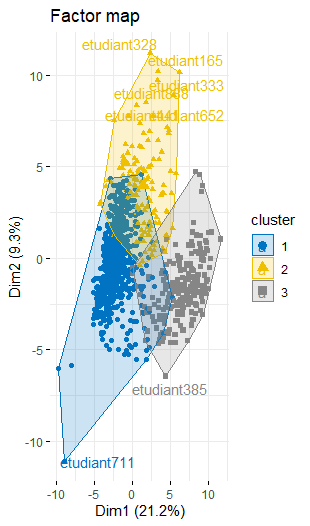
\includegraphics[scale=0.8]{hcpc.png} 
\caption[]{Ascending \ Hierarchical \ Classification \ of \ the \ individuals }
\end{center}
\end{figure}


\subsection{Results of HCHC} 

The cluster 1 is made of individuals sharing :

- high values for the variables  Galbant, Culpabilite, Ennuyeux, 
Stretchcing, Securite, Decouragement, Ralentissement, Lassitude,
Inconfort et Passivite (variables are sorted from the strongest).

- low values for variables like Progression, Transpiration, Performance,
Actif, Challenge, Plaisir, Objectif, Perseverance, Confiance en soi and Cardio 
(variables are sorted from the weakest).


The cluster 2 is made of individuals sharing :


-	high values for variables like Se defouler, Puissance, Competition, Technicite, Qualite, Energie, Confort, Muscle, Force and Intensite (variables are sorted from the strongest).

-	low values for the variables Sexy, Meilleur, Calme and Vital (variables are sorted from the weakest).


The cluster 3 is made of individuals sharing :


-	high values for variables like Progression, Actif, Performance, Challenge, Cardio, Partage, Plaisir, Depassement, Rapide and Efficacite (variables are sorted from the strongest).

-	low values for variables like Confort, Securite, Galbant, Douceur, Ennuyeux, Force, Maintien, Qualite, Beaute and Inconfort (variables are sorted from the weakest).


\newpage


\section{Classification}  %%%%  Testing the strength of clusters %%%%
 
 Nous avons séparer nos données en 3 parties :
- 80 \% des données pour le choix de l'algorithme de sélection .
- 20 \% des données pour tester le modele finale et éventuellement sélectionner les colonnes les plus importantes.

\subsection{Choice of Classification algorithm} 

 4 multiclass classifiers used : Supporting Vector Classifier
(SVC), Linear Supporting Vector Classifier
(LSVC), k-nearest neighbors 
(KNN) and  Logistic regression(logreg).

voici le graphique de la  performance de chaque modèle : 


\begin{figure}[H]
\begin{center}
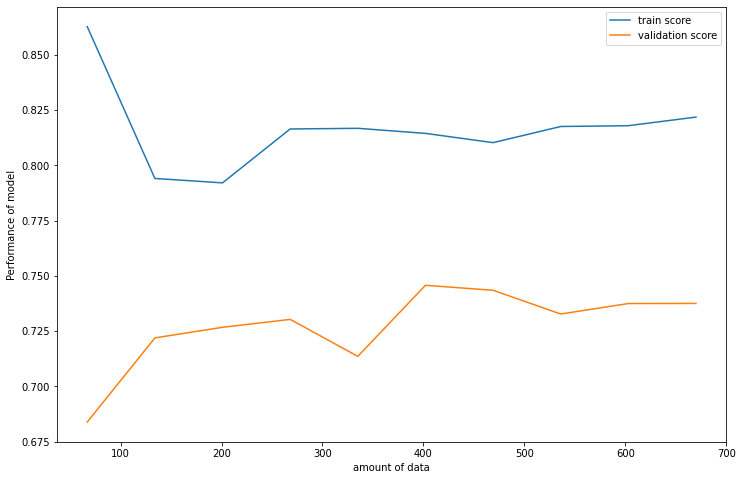
\includegraphics[scale=0.6]{learning_curve_1.png} 
\caption[]{ KNN \ learning \ curve }
\end{center}
\end{figure}

\begin{figure}[H]
\begin{center}
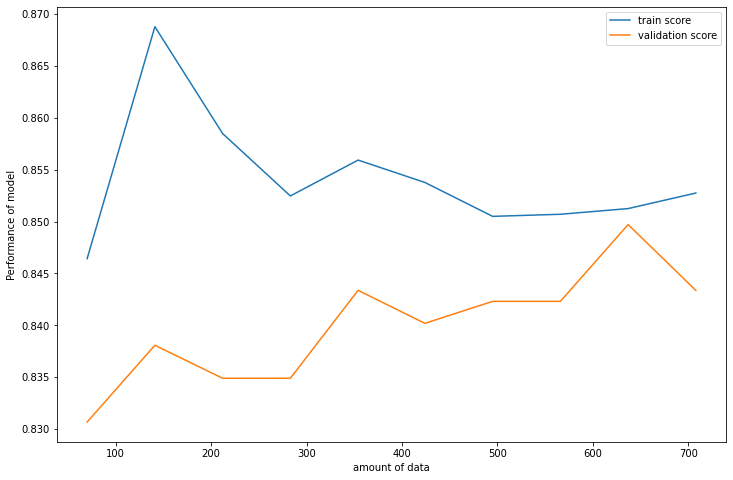
\includegraphics[scale=0.6]{learning_curve_2.png} 
\caption[]{ logreg \ learning \ curve }
\end{center}
\end{figure}

\begin{figure}[H]
\begin{center}
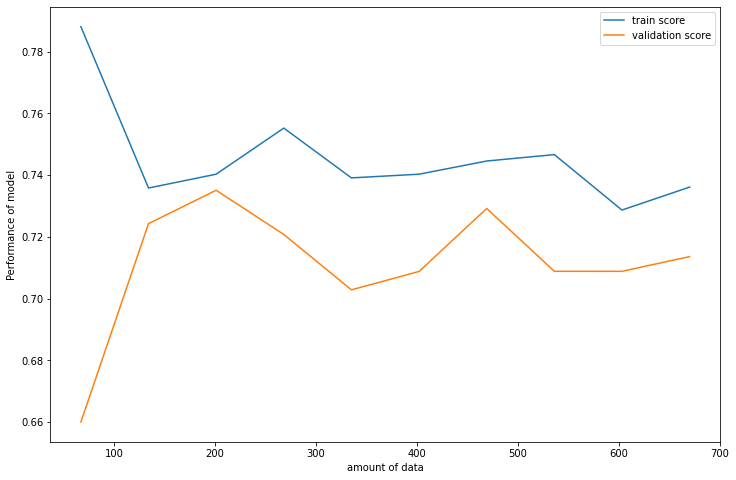
\includegraphics[scale=0.6]{learning_curve_3.png} 
\caption[]{ LSVC \ learning \ curve }
\end{center}
\end{figure}


\begin{figure}[H]
\begin{center}
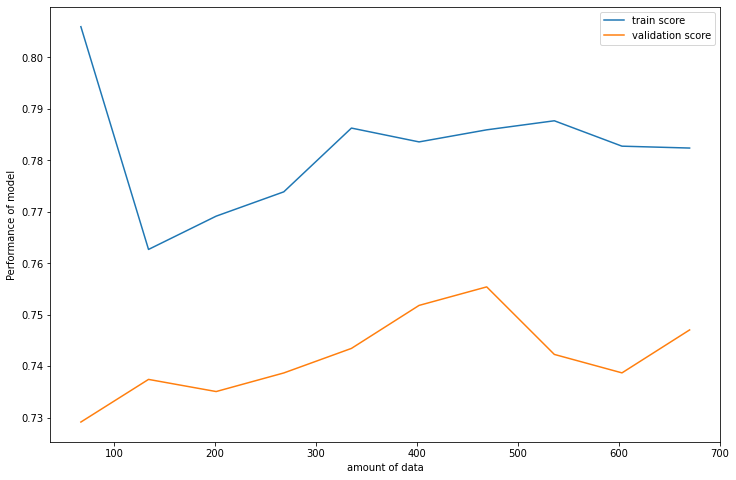
\includegraphics[scale=0.6]{learning_curve_4.png} 
\caption[]{ SVC \ learning \ curve }
\end{center}
\end{figure}



D'après les graphiques ci- dessous , la performance ou modele de lostigic Regression et SVC soit plus stable et meilleur que les autres modèles. On peut dire que les deux modèle ne sont pas en overfiting
(score train et score val sont proches) contrairement aux 2 autres.


Nous avons utliser  GridSearchCV pour optimser les hyperparametres du modele  logistic Regression. 
GridSearchCV nous permet de les meilleurs hyperpametre en comparant les différents performances 
 de chaque combinaison grâce a la technique de cross-validation.

La cross-validation consiste découper le jeu de données en k parties égales  ( ici k = 5). Tour à tour, chacune des k parties est utilisée comme jeu de test. Le reste (autrement dit, l’union des k-1 autres parties) est utilisé pour l'entraînement.

  
  
\subsection{Feature selection} 


Le graphique ci- dessous nous montre la variance de chaque features , nous avons constatons 4 valeurs 
remarquables 0.8 ou 0.06 ou 0.04 ou 0.02 qui pourront être le seuil .


\begin{figure}[H]
\begin{center}
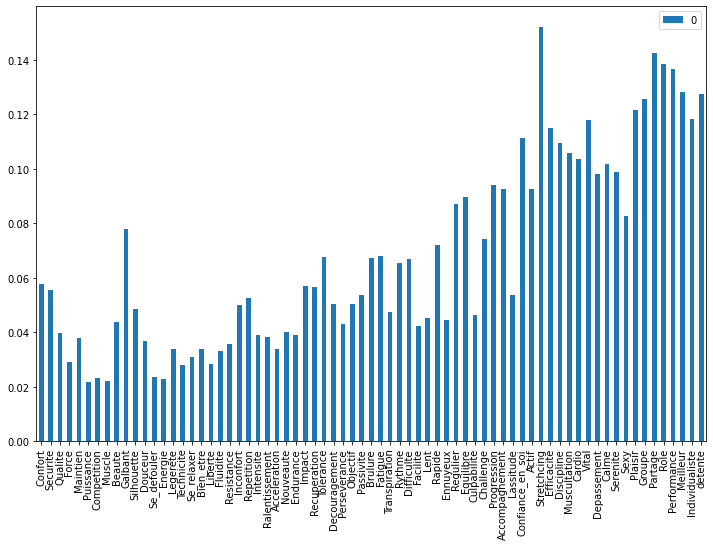
\includegraphics[scale=0.6]{barlot.png}
\caption[]{ variance\ of \ each \ features}
\end{center}
\end{figure}

Pour éliminer les valeurs inférieur à ce seuil , La fonction VarianceThreshold de scikit-learn a été utilisé.


Au final, le seuil fixé à 0.02 donne de meilleur résultats. Aucun  colonnes n'a été suprimée . 

\subsection{Results final model} 

\begin{figure}[H]
\begin{center}
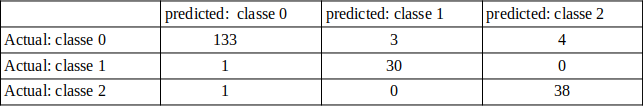
\includegraphics[scale=0.6]{confusion_matrix_1.png} 
\caption[]{  confusion \ matrix }
\end{center}
\end{figure}



\begin{figure}[H]
\begin{center}
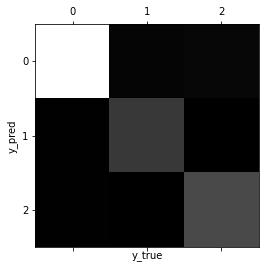
\includegraphics[scale=0.6]{confusion_matrix_2.png} 
\caption[]{confusion \ matrix}
\end{center}
\end{figure}

9 valeurs a été mal placées , le  recall\_score =  0.9640336366142818

 et f1-score =  0.9476814440703328


\section{Conclusion}
L'objectif principal du projet était de faire du  clustering sur nos données.
Grace au clustering HCPC , nous pouvons distinguer 3 types d'étudiants :

- les démotivés , ceux qui recherchent le bien-être et la simplicité dont certaines variables caractéristiques du cluster sont :  Culpabilite, Ennuyeux,  Decouragement, Ralentissement, Inconfort 

- Dans le deuxième groupe , on a ceux qui aiment les sports de combat comme la lutte, la boxe le MMA. il est caractérisé par ses mots : Puissance, Competition, Technicite, Qualite, Energie, Muscle, Force and Intensite 

- Le dernier groupe  se distingue par ses mots : Pro
gression, Performance, Challenge, Cardio, Partage, Depassement, Rapide and Efficacite. 
On retrouve ceux qui apprécient la course à pied et les activité de nature . 

En ce qui concerne la classification ,L'un des meilleur algorithme (SVM) a donné la valeur 0,722 de précision, 1,000 de rappel et 0,839 de FMeasure.(Par contre, l'ensemble de données de ce projet n'est pas assez grand.)

\begin{thebibliography}{9}

\bibitem{text}
\url{https://www.cairn.info/revue-staps-2018-2-page-99.htm}

\bibitem{text}

\url{https://solidarites-sante.gouv.fr/prevention-en-sante/preserver-sa-sante/article/activite-physique-et-sante}

\bibitem{text}
\url{https://e3s.unistra.fr/equipe/presentation/}

\bibitem{text}
\url{https://scikit-learn.org}

\bibitem{}
\url{https://fr.wikipedia.org/wiki/Analyse_en_composantes_principales}


\bibitem{text}
\url{http://www.sthda.com/english/}

\bibitem{text}
\url{http://www.sthda.com/english/articles/31-principal-component-methods-in-r-practical-guide/117-hcpc-hierarchical-clustering-on-principal-components-essentials/#algorithm-of-the-hcpc-method}


\bibitem{text}
\url{https://husson.github.io/teaching.html}


\bibitem{text}
\url{https://www.youtube.com/c/MachineLearnia}

\bibitem{text}
\url{}

\end{thebibliography}



\end{document}
